\section{Evaluation}
\label{sec:evaluation}
% One thing to think about in terms of presentation: In several places the
% wording sounds like we're changing (configuring) CrashSimulator to deal
% with this or that anomaly. I think it might be clearer to think of
% CrashSimulator as a black box that takes  as inputs:
% a) the program being tested
% b) a specific trace (or an input to that program, generating the trace on
% the fly)
% c) instructions for modifying the trace to simulate the anomaly, and
% d) instructions for  determining whether the application's response is
% acceptable.



CrashSimulator was evaluated as follows.
We implemented a prototype in a mix of Python 2 (5060 LOC) and C (2585 
LOC)\footnote{ Line count numbers are according to SLOCCOUNT~\cite{SLOCCOUNT}}.  
For a test
environment, we chose a virtual install of Ubuntu Linux 15.04 with a 32 bit 
kernel on i686 hardware.
We ran the tests on a 1.7 gHz core i7 system with 8GB of RAM. Our
implementation used {\tt ptrace} to interpose on the running program and
interject anomalous behavior into its execution.
We did not handle threaded programs and disabled ASLR and the kernel's vDSO 
to make replay easier.  As far as we are aware, none of these choices 
influenced the bugs that CrashSimulator can find, however the lack of support
for threaded programs obviously influences the programs we can test.  The 
only major impact these design choices had, was that our use of {\tt ptrace} 
slowed our prototype's performance (which will be discussed later) but made
constructing CrashSimulator easier.  Given appropriate anomaly information, 
our implementation of CrashSimulator can
test for anomalies that exist in other platforms and environments.  

Using this prototype, we answer the following questions about CrashSimulator:

\begin{enumerate}
   \item{[\ref{sec-env-bugs}] Do environmental bugs exist in widely used applications?}
   \item{[\ref{sec-complex}] Can CrashSimulator identify anomalies that require
       complex checkers?}
   \item{[\ref{sec-not-found}] What types of bugs could not be found using CrashSimulator?}
   \item{[\ref{sec-sorts-errors}] What sorts of errors does CrashSimulator make?}
   \item{[\ref{sec-perf}] Is CrashSimulator able to execute tests in a performant manner?}
%   \item{[\ref{sec-response}] What was the response to disclosing bugs found in CrashSimulator?}
\end{enumerate}



%15.04 with several modifications put in place to allow CrashSimulator to operate correctly. First, because
%CrashSimulator relies on an application's memory layout being the same across repeated executions, address space
%layout randomization must be disabled.  Second, the kernel's virtual dynamic shared object feature must be
%disabled.  This feature allows certain kernel data items (timestamps, kernel version information, etc.) to be stored
%in user space.  When the system calls that retrieve this information are made by an application they are instead
%intercepted and handled in user space -- a behavior that would preclude CrashSimulator from being able to interact
%with these calls.  Finally, a 32-bit Linux kernel and supporting environment were chosen.  While CrashSimulator
%could have been implemented on either a 32-bit kernel or a 64-bit kernel such a goal would have resulted in a great
%deal of duplicated effort around dealing with the low level differences between these two kernel versions.
%\emph{I've got a lot more I could talk about here but I'm not sure what info normally goes into this section}


%    \subsection{Limitations - What are CrashSimulator's Technical Limitations}

%The current implementation of CrashSimulator has the following limitations that could be addressed by future work.
%
%\paragraph{Coupling to Architecture}

%As some faults injected by CrashSimulator require low level access to the test system's hardware or operating
%system data structures there exists some degree of coupling between CrashSimulator and these components. One
%area of expansion for CrashSimulator is support for more processor architectures and more operating systems.
%CrashSimulator's test launcher as been designed in such a way that these improvements should be trivial to plug
%in once they have been implemented.
%
%\paragraph{Multi-threaded or Multi-process Applications}
%
%The current implementation cannot correctly replay applications that rely on multi-threading or
%multi-processing.  Is due to two factors.  First, the replay tool must be able to force some pre-determined
%order onto the threads or processes in order to prevent situations where the execution portion of a replay ends
%up requesting system calls in a different order than was recorded in the system call trace the system is
%attempting to replay.  Second, the tool needs to be able to correctly monitor multiple processes. {\tt ptrace}
%may have appropriate facilities for this task but they were not explored for this version of the tool.
%
%\paragraph{Multi-Platform Tracing Tool}
%
%While there are system call tracing tools available for most of the major operating systems available today
%there is not one tool that works across all of them.  This means that if CrashSimulator is going to be able to
%to work with traces from a given operating system, it will require specific parsing logic for the output of the
%tool used to record the traces.  Additionally, CrashSimulator requires that the tracing tools record all data
%passed into a system call and all data returned from the system call either as a return value or as some block
%of memory written into the calling process's memory.  It is possible that some system call tracing tools do not
%support this level of detail.


\subsection{Do environmental bugs  exist in widely used applications?}
\label{sec-env-bugs}

% Describe bug. Why is this attack badddk
% How crash simulator tests
% Show results
% Discuss  What should people think about it

Our first question focuses on whether there are any bugs of the sort that
CrashSimulator can find in popular applications.  After all, if such bugs
do not exist in practice, then there is no need for CrashSimulator.
To test whether such bugs exist in real programs, we 
chose two simple anomalies that could be tested in a large
array of programs.  We chose one file system anomaly and one network anomaly 
that used common API calls and thus had the potential to appear in
many programs.  We ran CrashSimulator on applications from GNU Coreutils and
on popular projects as is indicated by Debian's Popularity Contest~\cite{DebPopCon}.

\subsubsection{Unexpected File Types} 
\label{sec-file-type-bugs}
Providing unexpected types of files to
applications.

The first anomaly investigated occurs when an
application has to retrieve and process data from a file.  Linux supports
several ``special'' file types apart from the standard ``regular'' file type.
These include directories, symbolic links, character devices, block devices,
sockets, and First-In-First-Out (FIFO) pipes.  While these special files can
be operated on using the same system calls as regular files 
(such as {\tt read()} and {\tt write()}), they behave in very different
ways.  For example, {\tt /dev/urandom} is a character device that produces
an infinite amount of pseudo-random data when read.
If an application that reads the full contents of a file
before processing it is provided {\tt /dev/urandom}, it will fill memory
or disk and may crash the system~\cite{YumAptEndless}.
Correct execution in these situations
often requires that applications 
examine the files in order to ensure they are of an appropriate type.

{\bf Method.}  Identifying these bugs involves changing an application's
execution trace to emulate the application being provided a file type that is
unexpected.  For example, the {\tt sed} application, which modifies the contents
of a text file according to a provided command string, could be provided
a symbolic link, a directory, or a character device
instead.  CrashSimulator accomplishes this by identifying the calls to {\tt
  stat()}, {\tt fstat()}, or {\tt lstat()} that an application makes to examine
the file and then changes the trace to simulate that the regular file {\tt sed}
is expecting is actually one of the special file types.  If the application
responds to this injected information then there is the possibility that the
special file is being handled correctly.  If the application does not alter its
behavior then the anomalous condition is not being handled correctly.

% \cappos{Is this true in all cases?}
% Its true in the cases we have see so far.  This statement is based on our
% definition of what a "test" does as discussed in the approach details section.

{\bf Findings.}
Simulating these anomalies for each type of file
gave the results shown in Table~\ref{table:unexpectedtypes}. 

%\cappos{Is this true: We manually examined each application behavior
%simulated by CrashSimulator and verified it is consistent with the actual 
%behavior on the given file type.}
% I verified a subset of the results by providing actual "weird files"

For each application, CrashSimulator was invoked multiple times,
modifying the trace to simulate each of the non-standard file type anomalies.
Some of the applications opened multiple files; in these cases each
anomaly was simulated for each of the file arguments to the application.
%were used to examine the applications response to each of
%the listed file types. 
The columns of Table~\ref{table:unexpectedtypes} 
are labeled by the values that CrashSimulator inserts into
the return value of the {\tt stat()}-like call, corresponding to
different file type anomalies.
A result of ``Initial Value''
indicates that this type is the file type the application was provided when the
execution trace being replayed was recorded -- that is, a file of the type the
application was expecting.  A result of ``Recognizes'' indicates that the
application identified that it was being provided with an unexpected file type
and its execution diverged from the trace being replayed indicating that it was
potentially handling the unexpected file type correctly.  A result of ``Fail''
indicates that the application failed to recognize the presence of the unusual
file type because its execution did not diverge from the trace being replayed.
We manually examined a subset of the listed application behaviors simulated by
CrashSimulator and verified they were consistent with the actual behavior on the
given file type.

\begin{table*}[t]
    \scriptsize{}
    \begin{tabular}{l  l  |  l  l  l  l  l  l  l}
    \toprule{}
        Application & Condition Tested           & IFREG        & IFDIR        & IFCHR     & IFBLK    & FIFO      & IFLNK    & IFSOCK\\
\hline
        Aspell      & Dictionary File            & Initial Value  & Fail           & Recognizes  & Fail       & Fail        & Fail       & Fail\\
        Aspell      & File being checked         & Initial Value  & Fail           & Recognizes  & Fail       & Fail        & Fail       & Fail\\
        gnu-gpg     & secring.gpg                & Initial Value  & Fail           & Fail        & Fail       & Fail        & Fail       & Fail\\
        vim         & File being opened          & Initial Value  & Recognizes     & Recognizes  & Recognizes & Recognizes* & Recognizes & Fail\\
        nano        & File being opened          & Initial Value  & Recognizes     & Recognizes  & Recognizes & Fail        & Fail       & Fail\\
        sed         & File being edited          & Initial Value  & Fail           & Recognizes  & Fail       & Fail        & Fail       & Fail\\
        df          & /proc                      & Fail           & Initial Value  & Fail        & Fail       & Fail        & Fail       & Fail\\
        wc          & File being checked         & Initial Value  & Recognizes     & Recognizes  & Recognizes & Recognizes  & Recognizes & Recognizes\\
        du          & Directory being checked    & Recognizes     & Initial Value  & Recognizes  & Recognizes & Recognizes  & Recognizes & Recognizes\\
        install     & File being installed       & Initial Value  &
Recognizes     & Fail       & Fail      & Fail       & Recognizes &
Fail\\
        fmt         & File being formatted       & Initial Value  & Fail          & Recognizes  & Fail      & Fail       & Fail      & Fail\\
        od          & File being dumped          & Initial Value  & Fail          & Recognizes  & Fail      & Fail       & Fail      & Fail\\
        ptx         & File being read            & Initial Value  & Recognizes     & Recognizes  & Recognizes & Recognizes  & Recognizes & Recognizes\\
        comm        & Second file being compared & Initial Value  & Fail           & Recognizes  & Fail       & Fail        & Fail       & Fail\\
        pr          & File being read            & Initial Value  & Fail           & Fail        & Fail       & Fail        & Fail       & Fail\\
\hline
        readlink    & Link being evaluated       & \textbf{No file checks performed} & & & & & & \\
        unlink      & File being unlinked        & \textbf{No file checks performed} & & & & & & \\
    \bottomrule{}
    \end{tabular}
    \caption{Applications tested for their handling of unexpected file types.}
%\cappos{Aspell is much more interesting if there are different behaviors
%for different file opens tested.  Does another app have this?}
    \label{table:unexpectedtypes}
\end{table*}

The frequency of failed executions in our results indicate that many
applications make the assumption that they will only be used to process
regular files.  When this assumption does not hold the results of the
application's execution are hard to predict.  In many cases a denial of
service condition occurs in the form of the application ``hanging'' as it
attempts to incorrectly process the file.  This may happen harmlessly (such
as the case where an application blocks forever waiting for a {\tt read()}
call to retrieve non-existent data from an empty FIFO) or harmfully, as
happens in the case where an application attempts to read in and process an
``infinitely large'' file eventually filling available memory or disk
space~\cite{Cappos_CCS_08}. %\cappos{Please label the bugs w/ the impact.} 

%\cappos{there will need to be more discussion here.  I need more info about
%the results though, such as which bug does what...}

An interesting behavior we recognized when analyzing these results can be seen
in the last two applications listed in Table~\ref{table:unexpectedtypes}.  Each of these
applications correctly recognized when any file type other than its expected
file type was encountered.  This is because these applications are simply ``dumb'' wrappers
around the system calls they share a name with.  Essentially, they just hand
the specified file to their corresponding system call and, in the case of an
error, use {\tt perror()} to print the correct localized error message.  In
short, these applications pass their error handling responsibilities to the
kernel.

\subsubsection{Slowloris attack} Delaying network applications for extended
periods.

% Motivation - mentioned and addressed in other areas.  Effort in place to make package managers resiliant to this
% so that you can't be tricked into using old software
% All of these tools failed but we would expect that modern software like apt would be resiliant to it. We were unable
% to test several prominiant network programs because our tool cannot replay multi-threaded or multi-process programs


% Sentence at the end that says "now that we've seen that these issues are prevalent across major applications...

The second anomaly we examined using CrashSimulator
involves an application's behavior when it attempts to communicate over a network
with extremely long (on the order of minutes) response times.  At a low level,
applications retrieve data from a network socket by waiting for data to be
available and then reading it.  A key aspect of this approach is handling the 
situation where communication takes too long and should time out.
%detecting when the user should be notified of an issue because too much time has
%passed during the ``waiting'' step.  This takes the form of a timeout value
%which indicates after how much time the ``waiting'' operations should result in
%an error code that the application can handle.

{\bf Method.}
CrashSimulator can detect whether an application is vulnerable by modifying
the trace to change the time observed by the application to simulate large
amounts of time elapsing between network operations.
In this approach CrashSimulator determines
whether or not the application makes any effort to configure its network
communications with a timeout value. This is done by examining the presence or
absence of {\tt setsockopt()}, {\tt poll()} and {\tt select()} calls as well as
the timeout values that may or may not have been passed to them. Applications
that do not set the timeout are subject to the operating
system defined protocol timeout value (19 minutes on Linux).
Note that by properly manipulating the results of all
time-returning calls, CrashSimulator can simulate an execution where close to
the maximum timeout value occurred without actually spending any time
waiting.


We use CrashSimulator to analyze  network applications and libraries
that are amongst the most popular based on Debian's popularity contest 
ratings~\cite{DebPopCon}. 

%\begin{table*}[t]
\begin{table}[t]
  % Try apt-get, they have reported this as a bug
  \scriptsize{}
  \begin{tabular}{l | l}
    \toprule{}
	  {\bf Application}              & {\bf Analysis Result}\\
    wget                     & Overly long timeout supplied to {\tt select()}, vulnerable\\
    ftp                      & No {\tt poll()} or {\tt select()}, no timeout set, vulnerable\\
    telnet                   & {\tt select()} specifies no timeout, vulnerable\\
    urllib http              & No {\tt poll()} or {\tt select()}, no timeout set, vulnerable\\
    urllib ftp               & No {\tt poll()} or {\tt select()}, no timeout set, vulnerable\\
    ftplib                   & No {\tt poll()} or {\tt select()}, no timeout set, vulnerable\\
    httplib                  & No {\tt poll()} or {\tt select()}, no timeout set, vulnerable\\
    requests                 & No {\tt poll()} or {\tt select()}, no timeout set, vulnerable\\
    urllib3                  & No {\tt poll()} or {\tt select()}, no timeout set, vulnerable\\
    python-websocket-client  & No {\tt poll()} or {\tt select()}, no timeout set, vulnerable\\
    \bottomrule{}
  \end{tabular}
  \caption{Applications tested for their handling of extremely slow response
    times from the host with which they are communicating }
  \label{table:slowloris}
\end{table}
%\end{table*}


{\bf Findings.}
%As can be seen from the above results, all of the applications we examined were
%vulnerable to this sort of anomalous condition.  
 As Table~\ref{table:slowloris} shows, all of these
 applications %\cappos{include elapsed time needed to do a basic session.}
 were vulnerable to this sort of anomaly, with timeouts taking hours or
even days in some cases.
What's more, in the vast
majority of cases, the problem occurs because the application makes no effort to specify a
timeout value.  This means that the application is effectively falling back on
the operating system's maximum timeout value as defined for the protocol in
use.  This value is \emph{19 minutes} for the above applications as defined by
Linux for TCP sockets, allowing an
attacker to transmit one byte of data per timeout period to keep the
application alive.

This attack technique has been effectively exploited in the wild.  The {\tt 
slowloris} tool
allowed a single attacking host to successfully deny service to a vulnerable
web server with minimal bandwidth usage.  This attack worked by introducing
delays between the time headers were sent to the victim by an attacking HTTP
client.  Because many web servers at the time allowed large timeouts between
messages from the clients they were communicating with, one web client could
effectively tie up the resources of a web server for a long period of
time.
%As discussed above, the version of wget we examined is vulnerable to this sort
%of attack from the other direction.  Consider a malicious web server that
%monitors connecting clients with the goal of specifically targeting {\tt wget}.
%When it sees a connection from {\tt wget} it begins a reply process where
%messages are only sent every 800 seconds (remember that {\tt wget's} default
%timeout value is 899 seconds.  If {\tt wget} is not being actively monitored its
%transaction would take hours to complete.  This is particularly dangerous in
%situations where {\tt wget} is being run as a scheduled job.  It is very likely
%%that future iterations of the job could be kicked off before the intitial job
%completes.  At best there are now multiple iterations of the job conflicting
%with one another.  At worst, there could be 
This can cause a slow buildup of unending or long
lived jobs consuming resources and causing detrimental system 
behavior~\cite{Slowloris}.  Similar attacks can be used to indefinitely 
delay security updates to clients, leaving them vulnerable to 
compromise~\cite{Cappos_TR_08}.

%Because this attack has been seen in the wild, the developers of major projects
%have taken steps to ensure their applications are resiliant against it.  The
%{\tt apt} project is one such group.  We were unable to examine {\tt apt} and
%several other major network applications because of the prevlence of multiple
%threads and porcesses as a common pattern in handling network communications.
%We expect that CrashSimulator would find these major applications sufficiently
%protected.


{\bf Concluding Thoughts}
The results of the above analysis show that CrashSimulator is readily able to
identify novel bugs in widely used applications.  This includes
widely used tools, security-focused applications like {\tt gnu-gpg}, and 
host of popular network applications.  This is
because CrashSimulator focuses on identifying bugs that result from anomalous
conditions present in an applications environment.  CrashSimulator provides
a mechanism capable of testing a wide array of applications in a
repeatable, principled manner.
% For the unexpected file
%types bugs the fact that the anomalous conditions were handled in some cases but
%not in others indicate that an understanding that unexpected file types may be
%encountered is present in the applications' development communities but also
%that this understanding is incomplete.  The presence of these bugs in major
%security-centric applications like {\tt gnu-gpg} is of particular concern given
%the scrutany that its codebase has seen.  The fact that none of the applications
%we looked at by slowing network traffics correctly dealt with the situation
%indicates that these sorts of bugs may be a concern for even
%popular applications. 


%Thus we see that even very
%widely used applications are subject to failures due to unexpected file
%types.  The only major exception is those applications like {\tt mkdir},
%{\tt ls}, and {\tt chown}, that are thin wrappers on system calls.  This
%is because the operating system kernel handles error handling for those
%calls instead of the application

\subsection{Anomalies That Require Complex Checkers}
\label{sec-complex}
%\phyllis{Re-word this question?}

% Re-organize this to the same format as the above two sections
% Talk about doing manual source code analysis to identify interesting edge conditions

Having seen that CrashSimulator can detect many bugs with fairly 
simple anomaly injections and checks,
we wanted to understand whether CrashSimulator can identify more complex types
of misbehavior that crosses many system calls.
To do this, we examined the
way in which applications move a file in terms of the filesystem anomaly discussed in
section~\ref{subsec:anomalyexamples}.  This situation adds additional complexity that libraries and applications
frequently get wrong~\cite{PHPRenameBug,PythonShutilBug,NodejsCopyBug}.
%To come up with the
%instructions for how to simulate the anomaly, we examined the system 
%calls made by the {\tt mv} command and compared the behavior of other 
%tools.  We found that other tools made many errors when trying to move files.

%In Linux, the rename() system call will only move a file if the source and
%destination are on the same device.  This means that moving a file from a
%directory structure location on one storage device to a directory structure
%location on another device must be handled on a case-by-case basis by any
%application that relies on this operation.  

{\bf Method.}  To identify anomalies, 
we examined several libraries and found that {\tt mv} seemed
to handle cases that other tools failed to consider.  Following this, we 
used the trace of {\tt mv} as a template and created instructions to modify
the trace to simulate the anomalies that this program tests for.
The resulting anomalies that could be detected were as follows:
%Using these traces in CrashSimulator 
%\cappos{What is this?  I'm confused by what
%you are saying here.} that can determine whether or not a replayed
%execution of an application has performed all the necessary steps to
%successfully carry out a cross device move.  This analysis included manual
%review of system call traces of {\tt mv} moving a file across devices as well as
%analysis of its source code for interesting checks and edge conditions.  Each of
%the following are a ``step'' in the process of moving a file across devices that
%a well behaved application should carry out.


% Removed based on discussion
%\paragraph{Verify Destination is not Target of Source}
%
%In this condition, CrashSimulator confirms whether or not the application under test performs a check to ensure
%that the source file name is not a symlink pointing to the destination file name.  If this check is not
%performed, loss of data is possible due to removal or overwriting of the destination during the copy process
%resulting in the source symlink pointing to nothing. \emph{!!!! This is likely one that we would have trouble

%    detecting based only on system call behavior}
\paragraph{Source Replaced}

An application should make an effort to ensure that the file being copied is not 
replaced between the time it is initially examined and the time it is opened 
for copying.  Otherwise it could have been replaced by a file of a different
type, such as a character device.
%
%{\tt
%  mv} handles this situation by storing the inode number returned by an initial
%{\tt stat()} call and compares it to the inode number returned by an {\tt
%  fstat()} call made after the file has been opened for copying.  If the file
%has been replaced on the filesystem these inode numbers will differ and {\tt mv}
%will alert the user to the situation.  This strategy works because Linux does
%not truely remove a file until all applications that have a file descriptor to
%the file close it.  This means that if the file is intact after it has been
%opened, it is guaranteed to remain intact until the application finishes with it
%and calls {\tt close()} on its file descriptor. CrashSimulator is able to
%identify situations where the above saftey checks do not happen by monitoring a
%replay execution of a system call trace of an application moving a file across
%devices.  If the requisite system calls are not present then the application has
%not performed the file move safely and the execution is rejected.
To test whether applications are robust to anomalies involving source file replacement,
we developed a checker that monitors whether a series of safety checks
are performed and applied it to traces that simulated a cross-device move.
Failing to perform these checks often results in corruption of the file~\cite{PythonShutilBug}.

\paragraph{Preserve Xattrs}

Extended file attributes are used by modern
operating systems to store descriptive information about a file that cannot be
held by normal filesystem fields.  For example, an operating system can use
extended file attributes to store whether or not a file was downloaded from the
Internet -- important security information that used to warn
users if they are about to open a potentially unsafe file.  Apple's Gatekeeper
relies on extended file attributes to prevent applications downloaded from
untrusted developers from being executed without explicit user action~\cite{AppleCodeSigning}.
When copying a file,
an application should retrieve extended file attributes from the source
file and later apply them to the destination file.
%{\tt mv} handles
%preservation of these attributes by making the appropriate system calls to read
%all of the extended file attributes off of the source file and then applying
%them to the destination file.  Once again, CrashSimulator is able to determine
%whether or not an application has correctly preserved these attributes by
%monitoring a replay execution of an application moving a file across devices.
In this case, CrashSimulator used a checker
that watches for the application to make system calls
that read the extended file attributes from the source file (i.e. {\tt
  getxattr()}, {\tt lgetxattr()}, or {\tt fgetxattr()}) followed by system calls
that re-apply the attributes to the destination file (i.e. {\tt setxattr()},
{\tt lsetxattr()}, or {\tt fsetxattr()}).

\paragraph{Preserve Timestamps}

In order to truly copy a file from one device
to another an application needs to ensure that its metadata (such as the 
creation, modification, and access times) are preserved in the destination 
file.  
%{\tt mv} ensures that this
%occurs by making system calls that retrieve the POSIX timestamps associated with
%a file (content modification time, file status change time, and last access
%time) and apply them to the destination file.  
In this case, the checker monitors
%a replay execution in order to ascertain whether or not an application applies
whether when replaying a trace modified to simulate cross-device move,
the application applies
the appropriate timestamps to the destination file as part of moving a file
across devices by monitoring for a system call from the {\tt stat()} family to
retrieve the timestamps and system call from the {\tt utime()} family to apply
the retrieved timestamps to the destination file.
Failure to preserve timestamps has obvious
implications in records-keeping and archival situations as well as any situation
where a chronological record of file manipulations is important.  This can 
cause odd behavior in Makefiles, archival programs, and similar
software~\cite{NautilusTimestamps, SudoTimestamp}.

\paragraph{Copying Devices}

It is also important to check if a move would attempt to copy a special
character file like {\tt /dev/urandom} across disks.  As was discussed in the
previous section, many applications fail to examine the nature of a file before
operating on it.  So the file must be moved by creating a new device of the same
type at the destination, instead of reading from a potentially infinite device.
In our experience, applications that fail to perform this check end up
completely filling a disk or exhausting available memory -- sometimes causing the
system to become unresponsive.

%Table~\ref{table:crossdevice} lists the result of our analysis of several 
%popular applications and libraries that `move' files within a filesystem.  The
%column headings correspond to the short names listed for each of the previous
%paragraphs. A result of ``Correct'' indicates that the application or library
%function correctly performs the step described.  A result of ``Incorrect''
%indicates that the application failed to perform the step correctly or didn't
%make an effort to perform it at all.

 \begin{table}[t]
    \scriptsize{}
    \begin{tabular}{l p{1cm} p{1cm} p{1.2cm} p{1cm}}
    \toprule{}
        Application     & Source Replaced & Preserve Xattrs & Preserve Timestamps & Copying Devices\\
\hline
        mv              & Correct             & Correct         & Correct             & Correct\\
        mmv             & Correct             & {\bf Sec. Flaw} & {\bf Time
Loss} & Correct\\
        install         & Correct             & {\bf Sec. Flaw} & {\bf Time
Loss} & {\bf Fill Disk} \\
        perl File::Copy & Correct             & {\bf Sec. Flaw} & {\bf Time
Loss} & {\bf Fill Disk} \\
        shutils         & {\bf Corrupt}	& {\bf Sec. Flaw} 	& Correct             & Correct\\
        rust            & Correct             & {\bf Sec. Flaw} & {\bf Time
Loss} & {\bf Fill Disk} \\
        boost::copyfile & {\bf Corrupt}	      & {\bf Sec. Flaw} & {\bf Time
Loss} & {\bf Fill Disk} \\
    \bottomrule{}
    \end{tabular}
    \caption{Applications and libraries analyzed to determine whether or not
      they are able to correctly move a file from one device to another.
Incorrect entries are either missing the needed check or were ineffective.}
%\cappos{can we label them differently?}}
    \label{table:crossdevice}
\end{table}

{\bf Findings.}
As can be seen from the results in Table~\ref{table:crossdevice}, each of the
applications tested fails to perform one or more of the steps required to
successfully complete a cross-device move.  This is an unfortunate situation
because a failure to perform any one of these steps can result in negative
outcomes for the system as a whole.

Our results indicate that CrashSimulator is able to identify whether complex
operations are performed correctly in anomalous situations in
an array of popular programs.  
This includes the standard libraries for the programming languages Python,
Perl, and Rust, along with other widely used software.  This is true even
when many libraries have correct behavior in some cases, but not others.
CrashSimulator is effective at finding the anomalous behaviors in these
cases.
%These analysis rely on
%CrashSimulator's ability to compose sets of checkers that each deal with a step
%from the operation.  We have real world validation of this in the form of a bug
%report found on Python's bug tracker after we completed our analysis.  Python
%bug 15100 reports issues around the {\tt shutils} module's functions for copying files
%when they must do so across disks.  The report states the module doesn't do
%sufficient checking to prevent the race condition described in ``Source 
%Replaced''.
%CrashSimulator was able to correctly identify both that {\tt shutils} was
%not correctly performing the move operation and diagnose specifically that the
%``Source Replaced'' race condition was present.

\subsection{What types of bugs cannot be found using CrashSimulator?}
\label{sec-not-found}

Due to the level at which CrashSimulator works (the system call
level), it is not possible to find certain types of bugs.
CrashSimulator is not able to detect bugs that do not result from or
have a visible effect on the system calls an application makes.  An
example of this situation is applications mishandling a situation
around file moves where, due to a strange volume mounting arrangement,
the source directory is moved into itself.  In order to detect this
situation the application must make an effort to gather the full path
of both the source and destination and compare them.  While
CrashSimulator is able to observe some aspects of the ``gathering''
process (i.e. the {\tt stat()} or {\tt lstat()} calls) it is not able
to observe whether the application compares the strings.
CrashSimulator must see the correct actions via system calls (or
incorrect actions through the lack of them) to understand application
behavior.

%\emph{CrashSimulator could
%  detect this issue during a specially crafted execution which replays a trace
%  recorded where the issue was present.  I'm not sure how useful this would be
%  as presumably the while recording the trace the user would be able to directly
%  observe whether things happened correctly or not}
        
\subsection{What sorts of errors does CrashSimulator make?}
\label{sec-sorts-errors}
% Talk about both false positives and false negatives
% When and how they occur
% False negative would be checkers that aren't specific enough, or a given test case/checker is not included
% OR the system call trace does not include all of the information you need to know if something has happened
% Keep this short
%There are two types of errors that CrashSimulator makes. First, it can 
%incorrectly flag a situation as being an error (a false positive).  Second,
%it can fail to correctly detect an issue that actually occurs (a false 
%negative).  We discuss each situation in turn.
%
%{\bf False Positives.}
The primary source of false positives %(that is, CrashSimulator reports a failure
%in a situation where the execution should be accepted) for 
in CrashSimulator is an
application using a different sequence of system calls than a checker was
anticipating to implement a given operation.  CrashSimulator's
approach allows these situations to be easily corrected once identified.  This
is similar to the circumstance where an application's test suite is missing a
test, necessitating action by the developer to construct the missing test.

%In many cases a given operation can performed in several ways.  This means that
%a given operation may be correctly implemented by a set of system call sequences
%that differ from each other on a variety of dimensions.  
%In order to correctly
%classify applications that make use of alternative methods for a given operation
%the checkers must be able to check for several alternatives.

For example, consider GNOME's {\tt glib} file handling facilities.  When an
application makes use of these facilities to move a file across storage devices
the library itself correctly handles the behaviors described above as
making up a ``correct'' file move operation.  When we used CrashSimulator 
with the checkers described above to
analyze a minimal application that used {\tt glib} for a cross-device move,
we got reports stating that the application {\em did not} respond
correctly to the anomaly.
We found through manual examination of a
the system call trace that, while {\tt glib} correctly performs
the required behaviors, it does so using alternative system call sequences. 
Rather than using a sequence of
{\tt read()} and {\tt write()} calls, 
as our checker expected,
Glib creates a pipe and uses the
{\tt splice()} system call to copy the contents out of the source file, through
the pipe, and into the destination file.

Fortunately, as soon as false positives like this are discovered,
CrashSimulator's checkers can be modified to deal with alternative
approaches to handling an anomaly.
This approach is viable because there are a finite number of system calls, and a
given operation can be mapped to a manageable subset of system calls.  Given the
above example around moving files, consider the mapping from high level
``operation'' to the set of system calls that can implement it in
Table~\ref{table:stepsandcalls}.  Each of the steps in the operation map to a small
number of system calls and, in most cases, only one of the system calls is
necessary.  In situations where two system call sequences can correctly
implement the same operation CrashSimulator simply runs two checkers
in parallel and accepts the execution if either one ends in an accepting
condition.

\begin{table}[t]
    \scriptsize{}
    \begin{tabular}{l | l }
    \toprule{}
	    {\bf Operation}                                               & {\bf Potential System calls}\\
      Examine source file                                     & stat64(), lstat64(), fstat64()\\
      Examine destination file                                & stat64(), lstat64(), fstat64()\\
      Open source file                                        & open()\\
      Read contents of source file                            & read(), splice() with a pipe\\
	    List source file's & \\ ~~~~~extended file attributes             & listxattr(), llistxattr(), flistxattr()\\
      %Read contents of source file's extended file attributes & getxattr(), lgetxattr(), fgetxattr()\\
	    Read contents of source file's                    & \\
	    ~~~~~~~extended file attributes & getxattr(), lgetxattr(), fgetxattr() \\
      Open destination file                                   & open(), optionally unlink() the file first\\
      Write contents to destination file                      & write(), splice() with a pipe\\
	    Apply extended file attributes to & \\ ~~~~~destination file      & setxattr(), lsetxattr(), fsetxattr()\\
	    Apply proper timestamps to & \\ ~~~~~destination file             & utimens(), futimens()\\
	    Apply proper permissions & \\ ~~~~~to destination file            & chmod(), open() with a modeline specified\\
      Close the source file                                   & close()\\
      Close the destination file                              & close()\\
    \bottomrule{}
    \end{tabular}
    \caption{Each step of a successful cross-disk file move operation mapped to
      the system call or calls that can implement it}
    \label{table:stepsandcalls}
\end{table}


  \begin{table}
    \begin{tabular}{l l l}
      Application      & Detected Misbehavior      &   Result in execution\\
      od               & Fails to detect directory &   Fails reading from directory with read()\\
      ...              &  ...                      &  ... \\
    \end{tabular}
  \end{table}

  \subsection{Application Reactions in the Context of the Environment}

  \preston{
    In some cases, an application not detecting an anomalous condition doesn't
    mean the application has failed outright.  That is, sometimes the properties
    of the environment can ``save'' an execution that didn't detect a the
    anomalous condition.  A clear example of this is when an application that
    expects a regular file is handed a symlink instead.  This is the case when
    passing coreutils {\tt od} a symlink to a regular file rather than a regular
    file.  CrashSimulator indicates that {\tt od} does not detect this situation
    but because of the way symlinks work in Linux, {\tt od} is able to
    successfully process the target file anyway.  This approach could be
    problematic in environments where the properties of symlinks are not what
    {\tt od} expects.  Consider a hypothetical environment where the calls that
    {\tt od} uses like {\tt open ()} and {\tt read ()} access the contents of
    the symlink itself rather than the symlinks target.  In this case, the fact
    that {\tt od} does not detect that it has been handed a symlink would be
    problematic.}

  \preston{
    It is also possible that the properties of an application's environment can
    result in an anomalous condition is missed at the first detection
    opportunity but appears later in the execution.  An example of this is when
    coreutils {\tt od} is passed a directory rather than a regular file.
    CrashSimulator detects that {\tt od} does not recognize this condition when
    the input file is initially being opened and evaluated.  Instead, a future
    call to {\tt read ()} fails with an error code indicating that directories
    cannot be processed with {\tt read ()} in Linux.  Once again, the properties
    of the environment allow this anomalous condition to be detected at a later
    point rather than execution continuing and returning wrong results.
    Consider another hypothetical environment where {\tt read ()} calls are
    allowed on directories.  In such an environment {\tt od}'s use of {\tt
      read ()} would allow  cause execution to continue returning whatever data
    {\tt read ()} can access from a directory rather than bringing the
    anomalous condition to the attention of user.}

%{\bf False Negatives.}
%CrashSimulator can encounter false negatives (that is, CrashSimulator accepts an
%execution that it shouldn't) in three situations.  The first is that is hasn't
%been provided with the configuration necessary to test for the issue it missed.
%This is essentially the same as a ``missing testcase'' sort of situation that is
%common throughout testing methodologies.  CrashSimulator cannot identify issues
%it doesn't know how to look for.  The second situation is when a computational
%model is not constructed correctly and, as a result, misses an issue it should
%identify.  The third case, which relates to the first two, involves a situation
%where the trace level is inadequate to get enough semantic information to 
%make a correct judgment.  For example, system call tracing does not provide
%insight into computational actions that may be performed, such as an 
%application deciding to cache information in memory when it fails to open a 
%file.

\subsection{Is CrashSimulator able to execute tests in a performant manner?}
\label{sec-perf}

%\cappos{All of the performance numbers should be here.  I recommend having
%a graph with the normal run time on the x-axis and the replay speed on the
%y-axis.  It will be a scatter plot.  Each point will be one of the
%experiments you ran.}

One key attribute of successful testing tools is that they be able to
complete their tests in a timely manner.  If a tool takes too long to
complete its tests users will be less likely to run it frequently, or at
all, reducing the tools overall usefulness dramatically. To this end, the
performance of CrashSimulator was evaluated in order to determine whether
or not it was able to complete its test executions in an acceptable time
frame.  

{\bf Method.} Each of the following evaluations examines the completion
times for executions of the specified application in both
native and replay execution modes.


    \begin{figure}[t]
        \center{}
        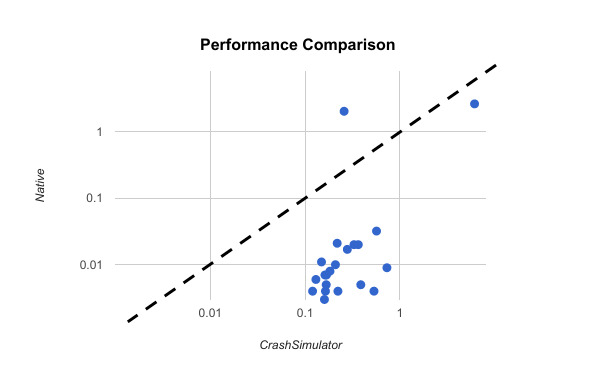
\includegraphics[scale=.5]{performance.png}
        \caption{\emph{This shows the run time difference between the
native program and CrashSimulator. The dashed line indicates equal
performance. }}

    \end{figure}


{\bf Findings.}
Overall, the performance of our CrashSimulator is usually about an order of
magnitude slower than executing the original program natively.  This is 
largely due to performance problems in our (unoptimized) prototype, 
primarily our utilization of {\tt ptrace}.  Tracing the program
with {\tt ptrace} adds up to a factor of 5x in overhead.  (This could
be removed with more efficient mechanisms like {\tt eBPF} or a loadable 
kernel module.)  Also the start up time of our prototype is high, due
to starting up the Python interpreter.


With a more optimized implementation, CrashSimulator could be much more 
efficient.  In fact, CrashSimulator will be more efficient than actually
running the program natively in many cases, since CrashSimulator only
replays the system calls.  This means that CrashSimulator does not need to
actually perform the calls which avoids the system call overheads, such as 
I/O.  Note that this already occurs for the {\tt du} program, because 
CrashSimulator need not actual perform any disk I/O.

Note also that natively testing the timeout of networked applications (not
shown) would take an extended period of time (at least as long as the allowed
timeout value).  CrashSimulator avoids this cost by simulating the fact that
time has progressed for future system calls.
%\cappos{Can we say something about the network timeout apps?}


%\cappos{I think the following should all get removed...  I don't understand the
%purpose}
%\paragraph{Discussion on network\_speedtest}
%    \begin{table}[H]
%        \scriptsize{}
%        \begin{tabular}{l  l  l  l}
%            \toprule{}
%                Execution Description & Native Eecution & Replay Execution\\
%                network\_speedtest & 0.024 & 2.407 \\
%                filesystem\_speedtest & 0.038 & 2.604 \\
%                mv (cross-disk file move) & 0.016 & 2.995 \\
%            \bottomrule{}
%        \end{tabular}
%        \caption{This sum total runtime of 20 runs of the listed application.}
%    \end{table}
%
%
%Sample application opens a TCP connection to an already running listener (netcat), sends a message, and
%exits. For simple applications like this, native execution is significantly faster than replay execution...
%
%\paragraph{Discussion on filesystem\_speedtest}
%
%This sample application create a new file with open(), writes a message to it, closes the file descriptor, and
%exit()'s. This test is particularly meaningful as it replicates a pattern of system calls that is used for in
%all sorts of applications in Linux...
%
%\paragraph{Discussion on mv}
%
%In addition to the newly constructed sample programs, performance values for replay of an execution of {\tt
%  mv} moving a file between two separate disks were recorded.  Results indicate that CrashSimulator is able to
%replay this operation in a similar time period to the time in which it is able to replay the dramatically
%simpler programs.  The fact that {\tt mv} makes an order of magnitude more system calls did not substantially
%increase replay time.
%\subsection{What was the response to disclosing bugs found in CrashSimulator?}
%\label{sec-response}
%
%
%After discovering the bugs in CrashSimulator, we filed bug reports with 
%different projects.  (To avoid unblinding our work, we do not link to the 
%bug reports here.)  The maintainers' response to these filings has been 
%positive.  Several projects have already applied patches to fix the bugs
%we reported.  For updated information about the number of bugs filed / fixed,
%we provide a blinded document~\cappos{refer to a webpage or google doc 
%that we will update}.
%
